\documentclass[12pt,a4paper]{article}
%\title{Software Requirements Specification}
%\date{December 14, 2015}
%\author{Aven Bross}
\usepackage[latin1]{inputenc}
\usepackage{amsmath}
\usepackage{amsfonts}
\usepackage{amssymb}
\usepackage{amsthm}
\usepackage{enumitem}
\usepackage[english]{babel}
\usepackage{fancyhdr}
\usepackage{chngpage}
\usepackage{geometry}
\usepackage{tabularx}
\usepackage{algorithm2e}
\usepackage[dvipsnames]{xcolor}
\geometry{legalpaper, portrait, margin=1.25in}

\usepackage{tikz}

\usepackage [autostyle, english = american]{csquotes}
\MakeOuterQuote{"}

\pagenumbering{gobble}

\begin{document}

\begin{center}

\begin{adjustwidth}{2em}{2em}
\begin{center}
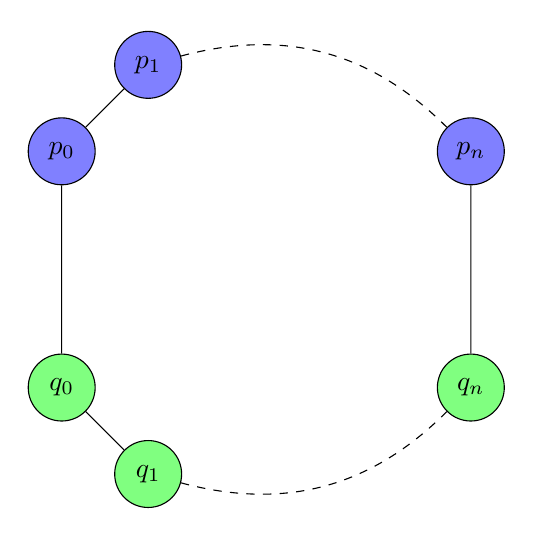
\begin{tikzpicture}[scale=1.5, every node/.style={circle, draw, minimum size=8.5mm, scale=1}]
  \node (p0) [fill=blue!50] at (150:2cm) {$p_0$};
  \node (p1) [fill=blue!50] at (120:2cm) {$p_1$};
  \node (pn) [fill=blue!50] at (30:2cm) {$p_n$};
  \node (q0) [fill=green!50] at (210:2cm) {$q_0$};
  \node (q1) [fill=green!50] at (240:2cm) {$q_1$};
  \node (qn) [fill=green!50] at (330:2cm) {$q_n$};
  \draw (p0) edge (p1);
  \draw (p1) edge [bend left] (pn) [dashed];
  \draw (q0) edge (q1);
  \draw (q1) edge [bend right] (qn) [dashed];
  \draw (p0) edge (q0);
  \draw (pn) edge (qn);
\end{tikzpicture}
\hfill\\
\footnotesize{Input to Poh algorithm.}
\hfill\\
\hfill\\

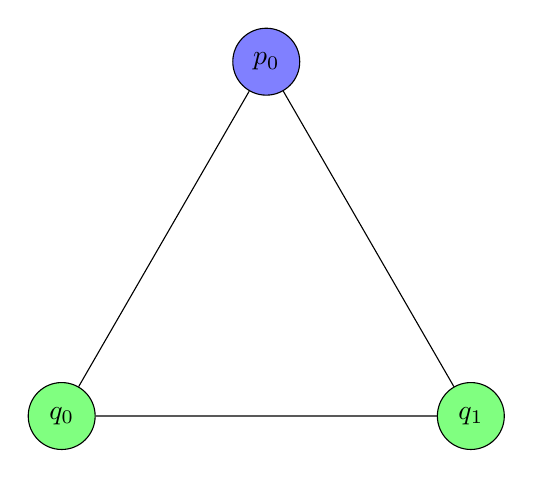
\begin{tikzpicture}[scale=1.5, every node/.style={circle, draw, minimum size=8.5mm, scale=1}]
  \node (p0) [fill=blue!50] at (90:2cm) {$p_0$};
  \node (q0) [fill=green!50] at (210:2cm) {$q_0$};
  \node (q1) [fill=green!50] at (330:2cm) {$q_1$};
  \draw (q0) edge (q1);
  \draw (p0) edge (q0);
  \draw (p0) edge (q1);
\end{tikzpicture}
\hfill\\
\footnotesize{Base case: A single triangle.}
\hfill\\
\hfill\\

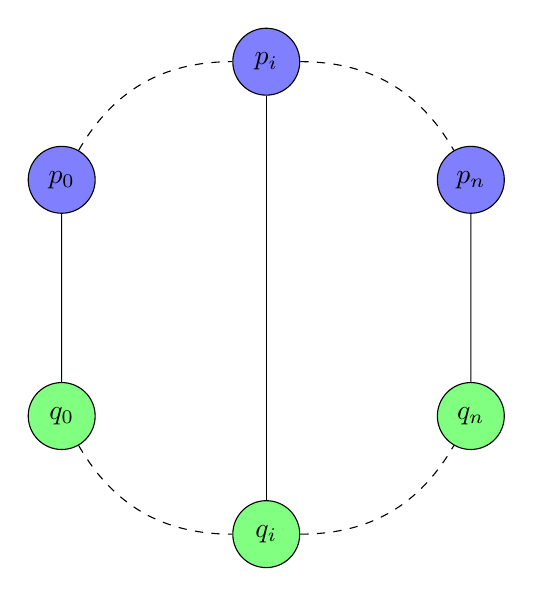
\begin{tikzpicture}[scale=1.5, every node/.style={circle, draw, minimum size=8.5mm, scale=1}]
  \node (p0) [fill=blue!50] at (150:2cm) {$p_0$};
  \node (p1) [fill=blue!50] at (90:2cm) {$p_i$};
  \node (pn) [fill=blue!50] at (30:2cm) {$p_n$};
  \node (q0) [fill=green!50] at (210:2cm) {$q_0$};
  \node (q1) [fill=green!50] at (270:2cm) {$q_i$};
  \node (qn) [fill=green!50] at (330:2cm) {$q_n$};
  \draw (p0) edge [bend left] (p1) [dashed];
  \draw (p1) edge [bend left] (pn) [dashed];
  \draw (q0) edge [bend right] (q1) [dashed];
  \draw (q1) edge [bend right] (qn) [dashed];
  \draw (p0) edge (q0);
  \draw (pn) edge (qn);
  \draw (p1) edge (q1);
\end{tikzpicture}
\hfill\\
\footnotesize{Case 1: Chord between paths.}
\hfill\\
\hfill\\


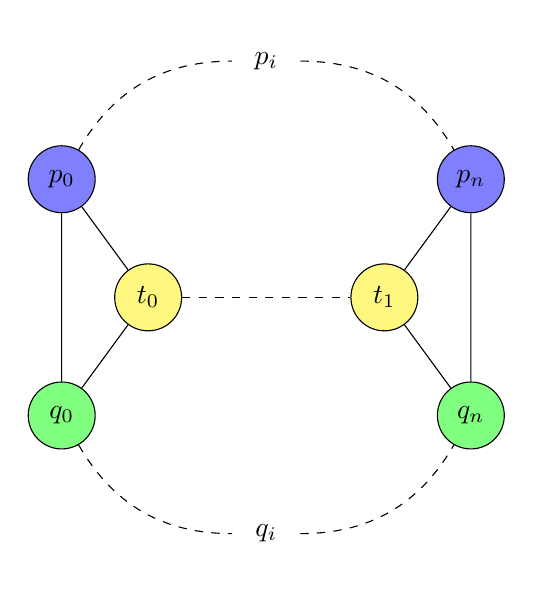
\begin{tikzpicture}[scale=1.5, every node/.style={circle, draw, minimum size=8.5mm, scale=1}]
  \node (p0) [fill=blue!50] at (150:2cm) {$p_0$};
  \node (p1) [draw=none] at (90:2cm) {$p_i$};
  \node (pn) [fill=blue!50] at (30:2cm) {$p_n$};
  \node (q0) [fill=green!50] at (210:2cm) {$q_0$};
  \node (q1) [draw=none] at (270:2cm) {$q_i$};
  \node (qn) [fill=green!50] at (330:2cm) {$q_n$};
  \node (t0) [fill=yellow!50] at (180:1cm) {$t_0$};
  \node (t1) [fill=yellow!50] at (0:1cm) {$t_1$};
  \draw (p0) edge [bend left] (p1) [dashed];
  \draw (p1) edge [bend left] (pn) [dashed];
  \draw (q0) edge [bend right] (q1) [dashed];
  \draw (q1) edge [bend right] (qn) [dashed];
  \draw (p0) edge (q0);
  \draw (pn) edge (qn);
  \draw (p0) edge (t0);
  \draw (q0) edge (t0);
  \draw (pn) edge (t1);
  \draw (qn) edge (t1);
  \draw (t0) edge (t1) [dashed];
\end{tikzpicture}
\hfill\\
\footnotesize{Case 2: Path between paths.}
\hfill\\
\hfill\\
\end{center}
\end{adjustwidth}

\end{center}

\end{document}